%!TEX root = ../thesis.tex
\chapter{Proposed Design} % (fold)
\label{ch:design}
\todo[inline]{First and second iteration}

\section{Acquiring and Mining Data for Personalisation}

The \cite{DCMI} proposes 15 meta data elements, i.e.\ Title, Creator, Subject, Description, Publisher, Contributor, Date, Type, Format, Identifier, Source, Language, Relation, Coverage and Rights.

categories predefined, but must be updated -- later the recording of the user behaviours can supply these category choices. Also they should be based on the root terms presented in \cite{10-1-1-19-5583}.
%Web personalisation is by \cite{DataMiningMobasher} divided into phases of data collection and preprocessing, pattern discovery and evaluation, and applying the discovered knowledge in real-time to mediate between the user and the Web.

This section will describe the necessary data mining before it is possible to apply personalisation on the digital newspaper.
\begin{quotation}
%	``Personalization technology enables the dynamic insertion, customization or suggestion of content in any format that is relevant to the individual user, based on the user’s implicit behaviour and preferences, and explicitly given details.
%	This can be dissected as:
%	`Personalization technology enables the dynamic insertion, customization or suggestion of content' – personalization doesn’t just have to be product recommendations: it can also include inserting any content like images or text (e.g. displaying a golf-orientated banner for a returning golf supplies buyer), or customizing content that is already there (e.g. `Hi Joe, we've got some great movie suggestions for you!').
%	`$\cdots$ in any format' – it isn’t restricted to the web. It can be implemented for any medium or touchpoint, such as emails, apps, instore kiosks, etc.
%	`$\cdots$ that is relevant to the individual user, based on the user's implicit behaviour and preferences, and explicitly given details' – finally, the most important part. Personalization uses both implicit and explicit information, derived in two ways. Firstly, a visitor might explicitly declare some information, such as their gender or date of birth.''
\end{quotation}
%\todo[inline]{definition from elsewhere than wikipedia}

\todo[inline]{Won Kim, ``Personalization: Definition, Status, and Challenges Ahead'', Journal of Object Technology, Volume 1, no. 1 (May 2002), pp. 29-40}


\todo[inline]{spacial, temporalt, topics (content) -- en distribution over topics -- (probabilistisk model -- distribution af ord -- referer til en lda model), lidt det samme at tale om et billede og musik.}
Reference: \cite{BleiTopics}



\subsection{Implicit and Explicit Data Collection}
\cite{MagdaliniWebMining}


\todo[inline]{Introduce collaborate filtering}
\todo[inline]{Introduce relevance feedback (click on article, time spend reading it and scroll)}
\todo[inline]{Read ``Personalization Techniques and Their Application.pdf''}

using hash of url as ids.

looking for images and videos in the article.

\subsection{Word tagging}
tagging: maxent\_treebank\_pos\_tagger, Treebank Part of Speech Tagger (Maximum entropy) -- sikkert upenn corpus.
%upenn\_treebank.pdf

alternativt: Treebank Part of Speech Tagger (HHM)


wordnet\_enrich: ``W-kmeans: Clustering News Articles Using WordNet'', 116262780379.pdf

wordnet sammensatte ord

citep ``Text Classification Using WordNet Hypernyms.pdf''
hypen density. This is better in 116262780379.pdf

using nouns and adjectives NOT nouns and verbs as in ``Text Classification Using WordNet Hypernyms.pdf''


tagging på feeds er givet fra feedets navn. Kan bruges til at verificere min classification.



Opbygge en database med articler og bruge det som basis for similarity queries.
wordnet\_ic Information Content: Load an information content file from the wordnet\_ic corpus.
\begin{lstlisting}[caption=cap,label=lst:lab,float=htbp]
	>>> from nltk.corpus import wordnet_ic
	>>> brown_ic = wordnet_ic.ic('ic-brown.dat')
	>>> semcor_ic = wordnet_ic.ic('ic-semcor.dat')
	>>> dog.res_similarity(cat, brown_ic)
	7.9116665090365768
	>>> dog.res_similarity(cat, genesis_ic)
	7.1388833044805002


explain SELECT MAX(sim) as max_val FROM `hypens` WHERE hypen1 IN ( .... ) AND hypen2 IN ( ... ) GROUP BY hypen1;
+----+-------------+--------+-------+---------------+----------+---------+------+----------+-------------+
| id | select_type | table  | type  | possible_keys | key      | key_len | ref  | rows     | Extra       |
+----+-------------+--------+-------+---------------+----------+---------+------+----------+-------------+
| 1  | SIMPLE      | hypens | index | hypen1_2      | hypen1_2 | 126     | NULL | 49472237 | Using where |
+----+-------------+--------+-------+---------------+----------+---------+------+----------+-------------+
\end{lstlisting}


\cite{21172_ftp.pdf} presents ontology levels from front page (overview) to a specific subject providing the ability to browse articles based on different levels delimitation. Also, that the most interesting articles should be placed on the front page and other relevant articles within each category. The same ability is provided through the rough overview on the front page, with the top articles of each section and the possibility to specify each section on the the preferred level of ontology. E.g.\ if the user wants articles from the broad category of business, this category can be chosen and through the time spend on diverse articles, the system will learn that this is the preference of the user. That is, of cause only given that the user acts his preference. Also, the Wordnet enriching of the articles works on the basis of ontology levels in the hierarchy of Wordnet structure.

It should as \cite{21172_ftp.pdf} proposes be possible to get the standard edition of the newspaper if the user does not need personalised news. This could be done by simply turning off the implicit recording of the user behaviour -- this will handle some privacy issues as well.

\section{Interface}
\cite{NielsenWeb} on how users read on the web ``They don't. People rarely read Web pages word by word; instead, they scan the page, picking out individual words and sentences.''

``2. PDF Files for Online Reading:
Users hate coming across a PDF file while browsing, because it breaks their flow. Even simple things like printing or saving documents are difficult because standard browser commands don't work. Layouts are often optimized for a sheet of paper, which rarely matches the size of the user's browser window. Bye-bye smooth scrolling. Hello tiny fonts.
Worst of all, PDF is an undifferentiated blob of content that's hard to navigate.''

``4. Non-Scannable Text:
A wall of text is deadly for an interactive experience. Intimidating. Boring. Painful to read.
Write for online, not print. To draw users into the text and support scannability, use well-documented tricks:
\begin{itemize}
	\item subheads
	\item bulleted lists
	\item highlighted keywords
	\item short paragraphs
	\item the inverted pyramid
	\item a simple writing style, and
	\item de-fluffed language devoid of marketese.
\end{itemize}
''

``5. Fixed Font Size
Respect the user's preferences and let them resize text as needed. Also, specify font sizes in relative terms — not as an absolute number of pixels.''
\cite{NielsenOnlineReading}

\subsection{Typeface}

Colour scheme: \url{http://colorschemedesigner.com/#0042b1Tw0w0w0}

\begin{figure}[h!tp]
	\centering
		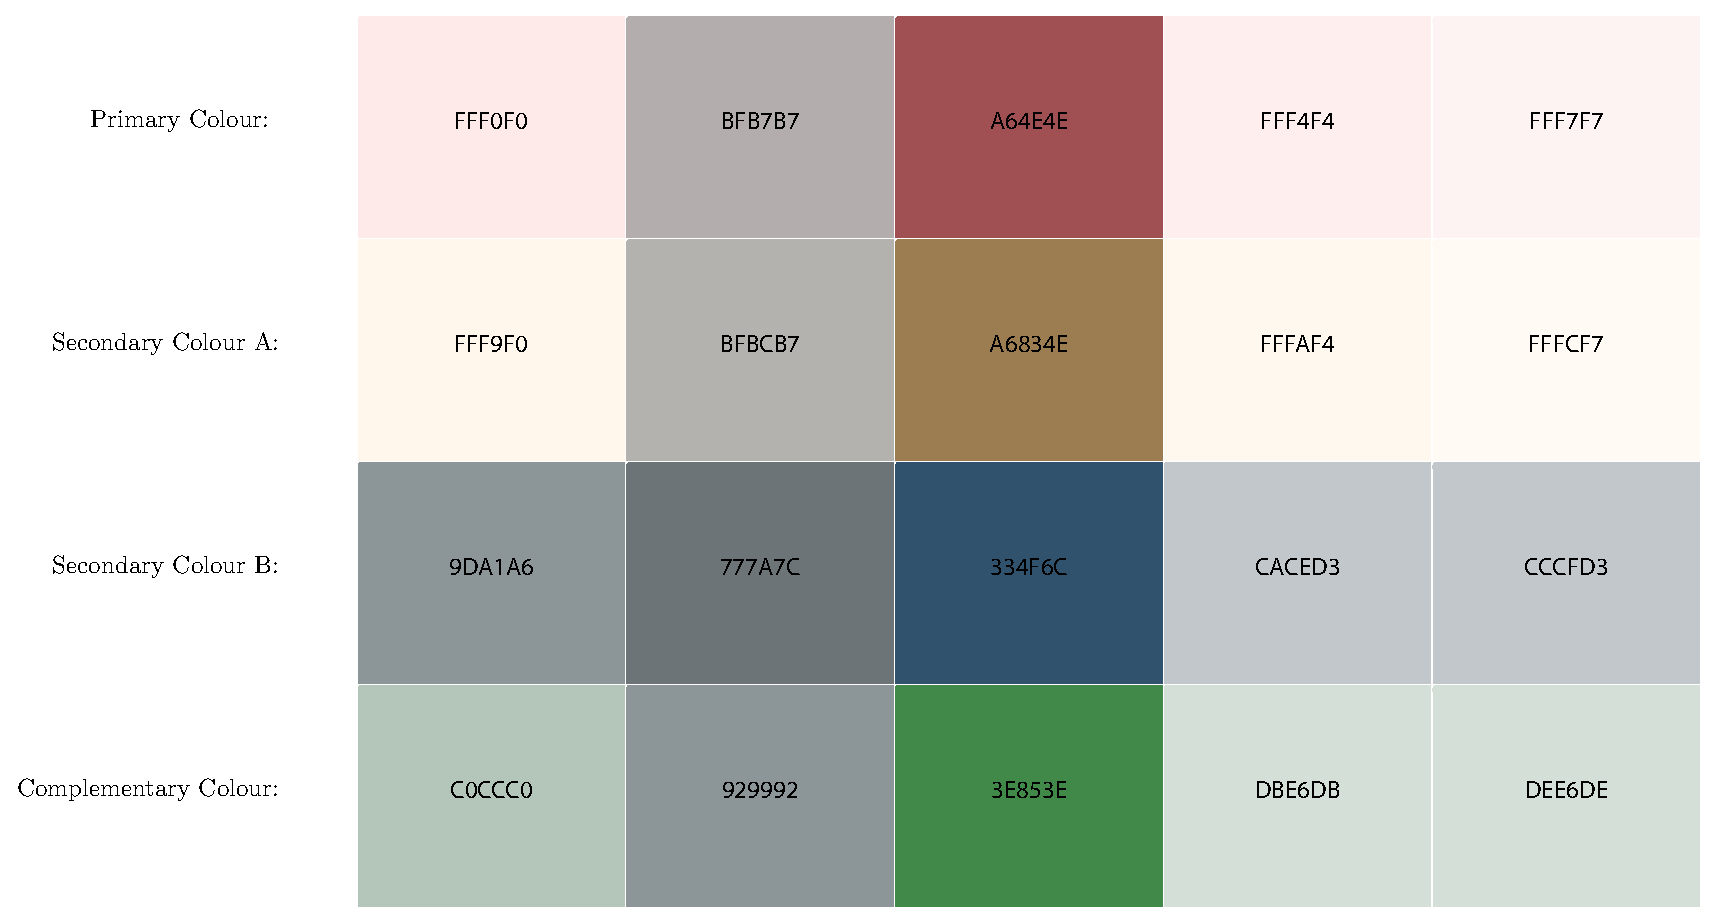
\includegraphics[width=.45\textwidth]{img/colour-scheme.eps}
	\caption{Colour scheme of the interface \protect\cite{colorschemedesigner.com}}
	\label{fig:colour-scheme}
\end{figure}
\todo[inline]{colorschemedesigner.com citep}

\section{Constraints}
The constraints can be divided into groups: layout-/content-based, global/topic/neighbouring, 


Technical argumentation for choices.
Business case argumentation for choices (user needs).
Reference to written articles about design choices -- navigation: sections + headlines, 

\subsection{Layout Constraints}
first focus: layout + one sections

3? columns
images/no image
base layout



\subsection{Content Constraints}
Content similarity relationships:
article vs. neighbouring articles
article vs. containing section/topic
article vs. whole newspaper

breaking
``[...] it was found that the best eight-item  mix within an issue was not necessarily composed of the eight highest-readership items in that issue.'' \cite{EditorsDilemma} (maximum audience coverage, which is no longer an issue due to personalisation)

\begin{align*}
\mathcal{C} &=	\begin{Bmatrix}
					\texttt{all\_different}(a_i),\\
					\texttt{sim}(a_i, a_{i+1}, 0.7, 0.9), \\
					\texttt{sim}(a_i, a_{i-1}, 0.7, 0.9), \\
					\texttt{sim}(a_i, a_j, 0.3, 0.9)
					%artists_i \ne artists_{i-1} \wedge artists_i \ne artists_{i+1},\\
					%album_i \ne album_{i-1} \wedge album_i \ne album_{i+1},\\
					%\texttt{all\_different}(place_i),\\
					tempo_i < tempo_{i+1} + 10 \wedge tempo_i < tempo_{i-1} + 10 \wedge\\
					tempo_i > tempo_{i-1} - 10 \wedge tempo_i > tempo_{i+1} - 10,\\
					%tempo_i < + 5 \cdot length \cdot tempo_j \wedge\\
					%tempo_i > - 5 \cdot length \cdot tempo_j\ \textbf{for}\ i \ne j,\\
					%keys_i = keys_i \vee keys_i = keys_i \pm 1 \vee keys_i = keys_i \pm 12
				\end{Bmatrix}
\end{align*}


\todo[inline]{AIRussel p. 207 preference constraints. can often be encoded as costs on individual variable assignments. Solved either path-based or local.
p. 216 Minimum-remaining-values, p. 217 Least-constraining-value.}

\todo[inline]{Figure of the system design: Model (user model + meta data + constraints), View (layout + inteactions), Control (cp)}

% section design (end)